% !TEX root = main.tex

\section{处理器}
\subsection{处理器概述}
计算机五大组成部分:[控制器+数据通路/运算器](处理器)、存储器、输入、输出
\begin{itemize}
	\item 操作元件:组合逻辑电路,所有操作元件都必须从状态元件接受输入,并并将输出写入状态元件
	\item 状态元件:时序逻辑电路,只有状态元件可以存储信息
\end{itemize}
\begin{definition}[寄存器组(Register File)]
包含
\begin{enumerate}
	\item 两个读端口(组合逻辑):busA和busB读入地址,经过一个取数时间(AccessTime)后,两条线有效
	\item 一个写端口(时序逻辑):写使能为1且时钟边沿到达
\end{enumerate}
要输入信号在寄存器的输出端才有效
\end{definition}
\par 一个时钟周期就是一个节拍。
\par PC和指令寄存器的位数分别取决于存储器的容量和指令字长。

\subsection{数据通路的建立}
CPU执行指令主要分为两个阶段
\begin{enumerate}
	\item 取指阶段(公共操作):
	\begin{itemize}
		\item 取指令:经过一个clk-to-Q(门闩延迟),PC得到新值,经access time后得到当前指令
		\item $PC\gets PC+\Delta=PC+4$
		\item 译码
	\end{itemize}
	\item 执行阶段:
	\begin{itemize}
		\item 主存地址运算
		\item 取操作数
		\item 算术逻辑运算
		\item 存结果
		\item 判断检测异常事件
		\item 若有异常,则自动切换到异常处理程序
		\item 检测是否有中断请求,有则转中断处理
	\end{itemize}
\end{enumerate}
\begin{figure}[htbp]
\centering
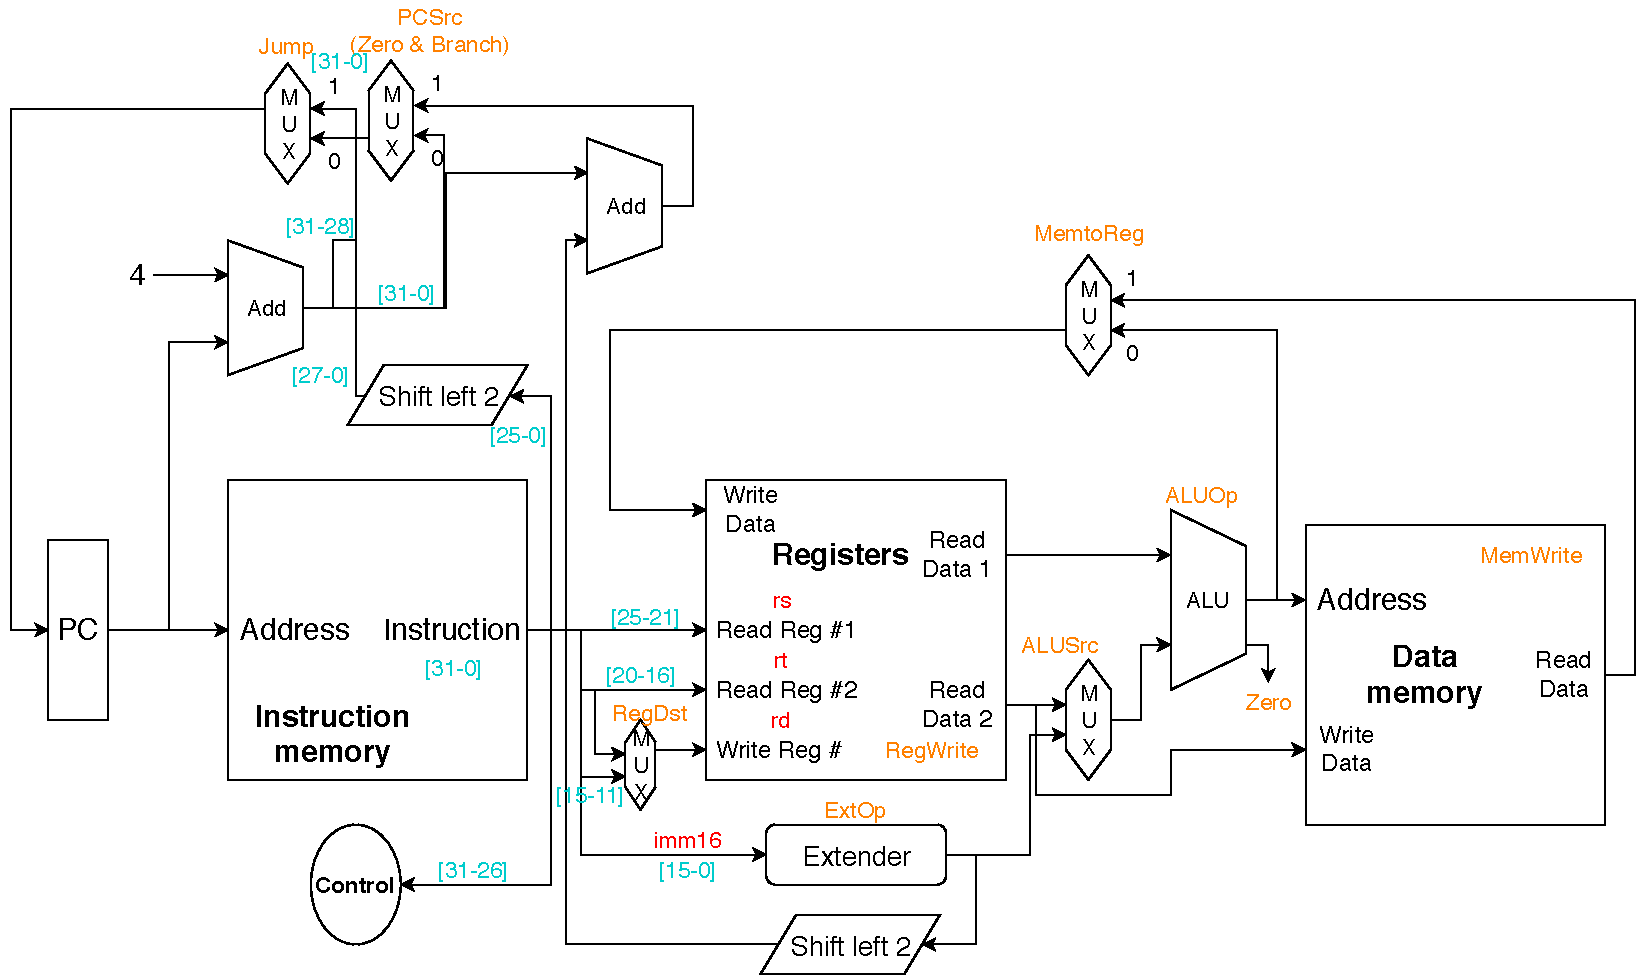
\includegraphics[width=\linewidth]{fig/Datapath_All.pdf}
\caption{MIPS基本数据通路}
\end{figure}
\par MIPS中三类基本指令:R-type、I-type、J-type,基本数据通路如下
\begin{enumerate}
	\item 加减 \verb'add/sub rd,rs,rt'
\begin{figure}[htbp]
\centering
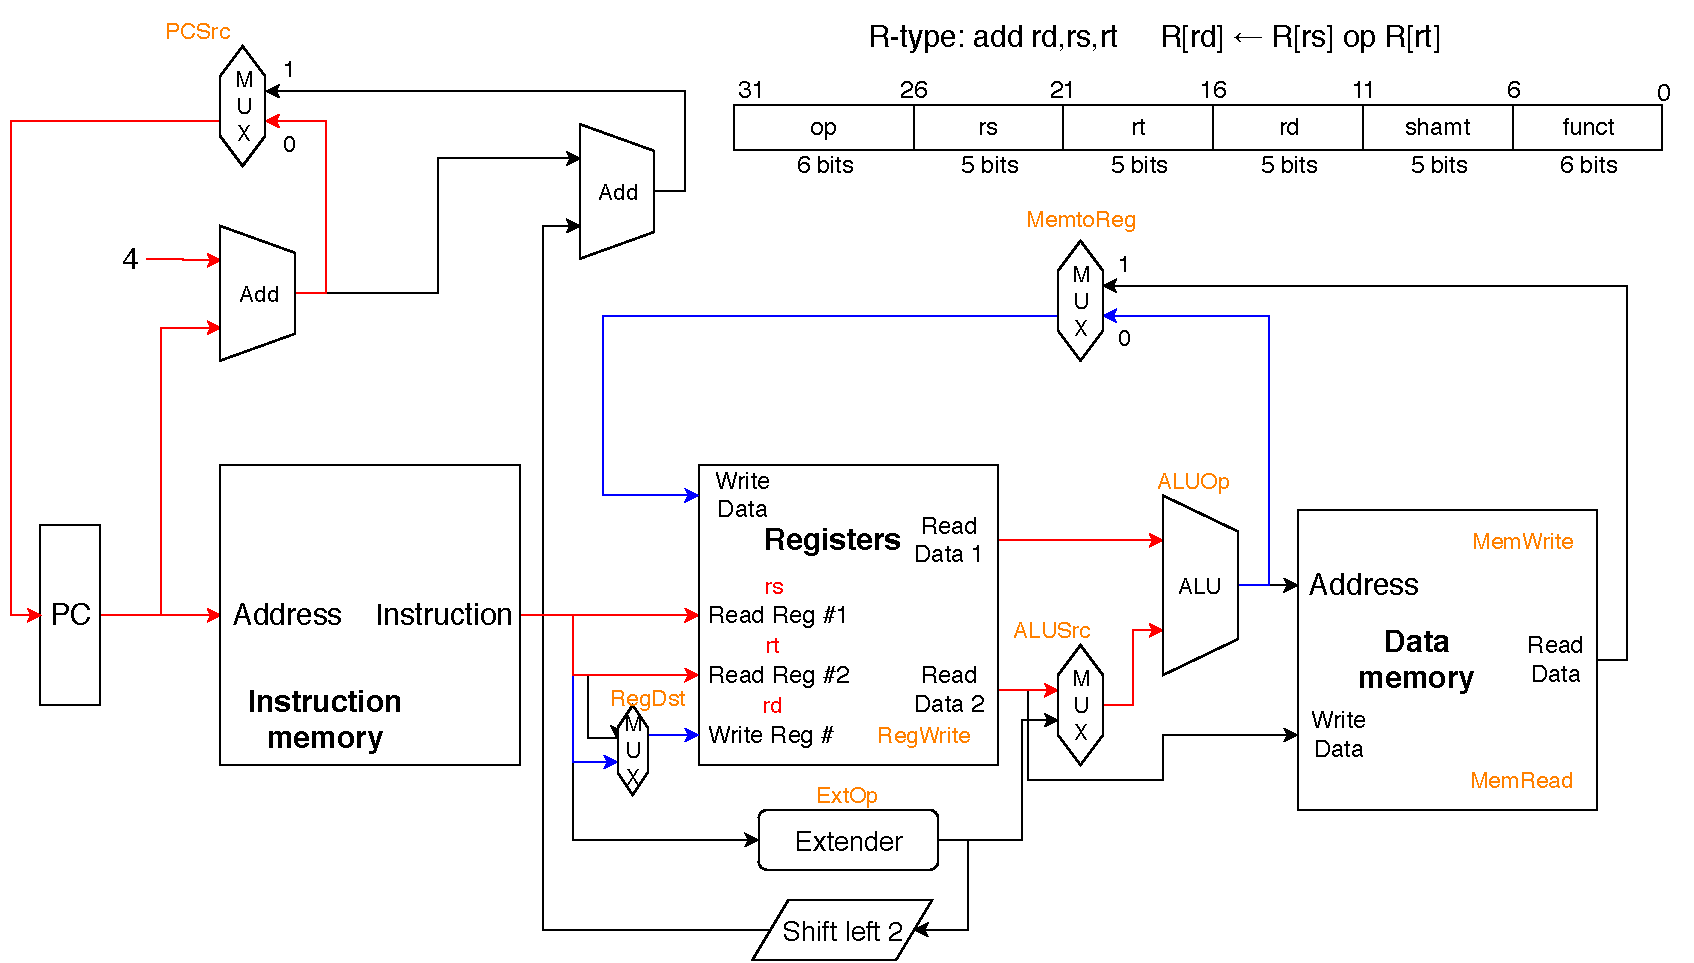
\includegraphics[width=\linewidth]{fig/Datapath_add.pdf}
\caption{add/sub通路}
\end{figure}
	\item 或立即数 \verb'ori rt,rs,imm16':零扩展
\begin{figure}[htbp]
\centering
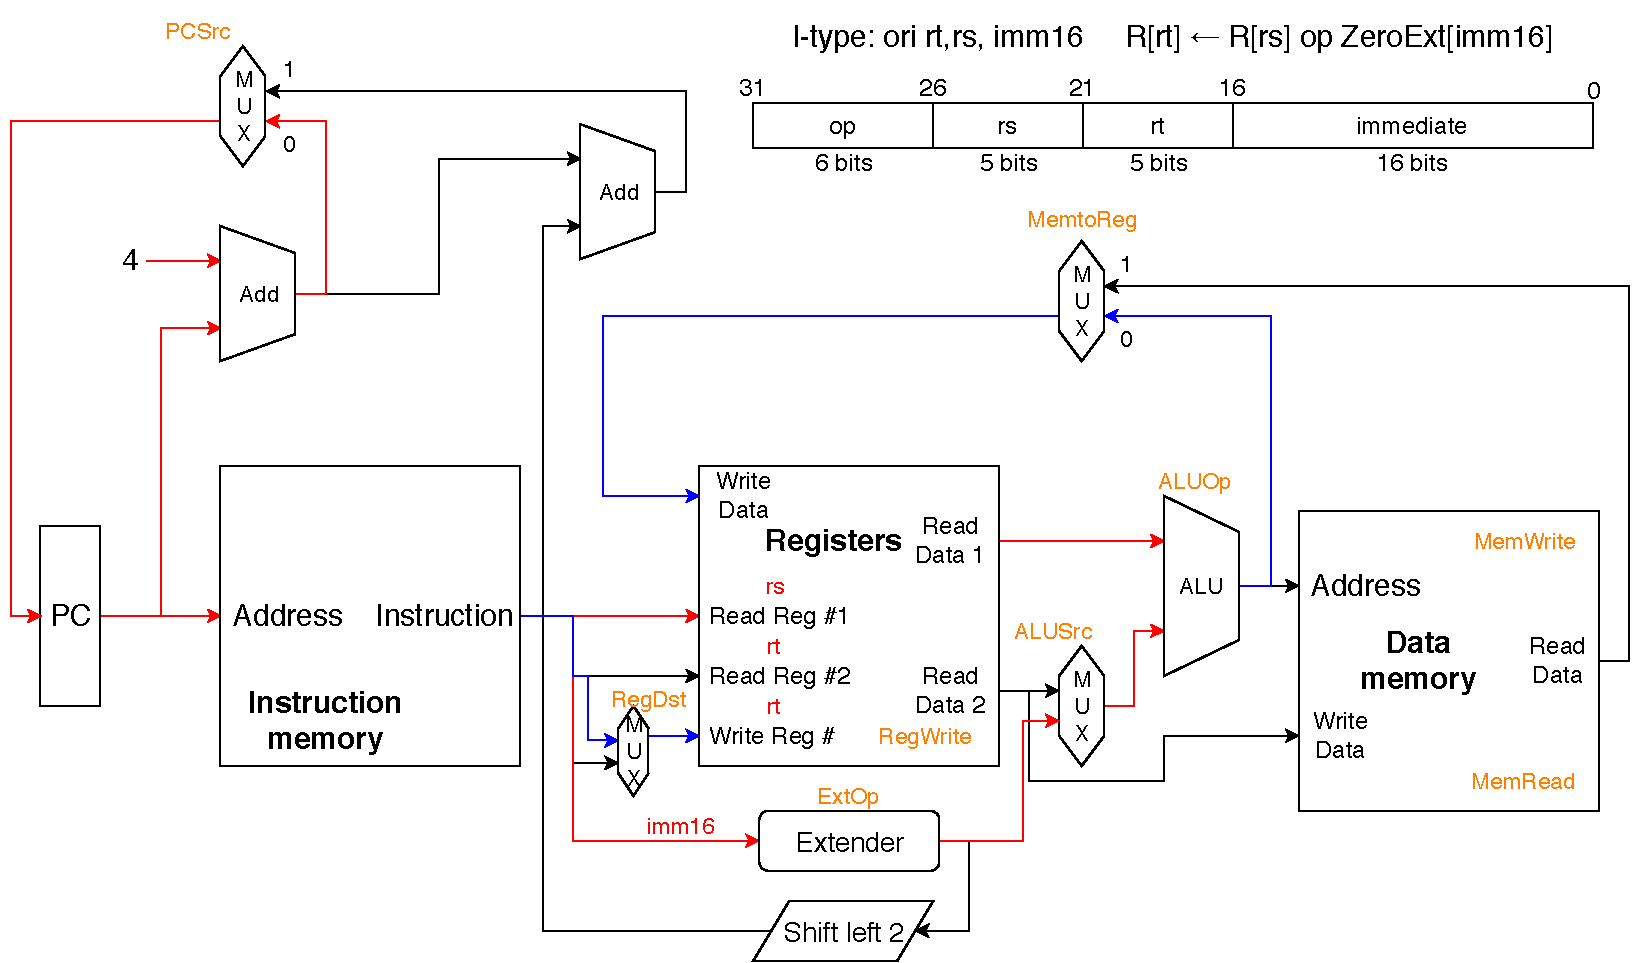
\includegraphics[width=\linewidth]{fig/Datapath_ori.pdf}
\caption{ori通路}
\end{figure}
	立即数需要零扩展(ZeroExt)为32位
	\item 存 \verb'lw rt,rs,imm16':符号扩展
\begin{figure}[htbp]
\centering
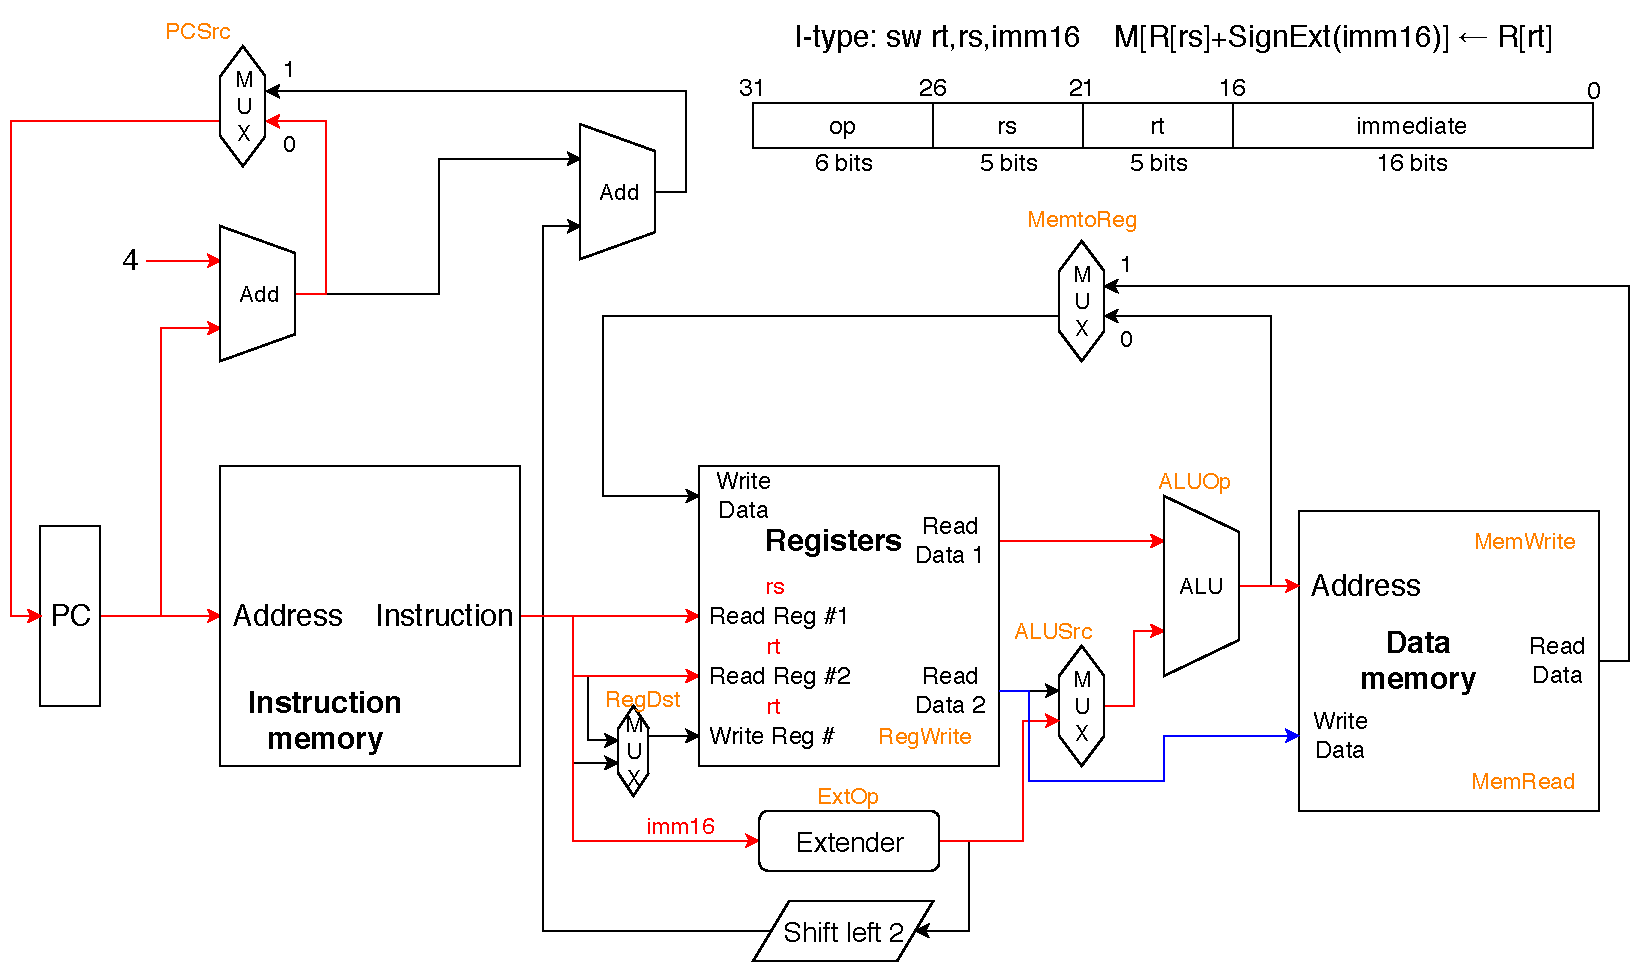
\includegraphics[width=\linewidth]{fig/Datapath_sw.pdf}
\caption{sw通路}
\end{figure}
	\item 取 \verb'sw rt,rs,imm16':符号扩展
\begin{figure}[htbp]
\centering
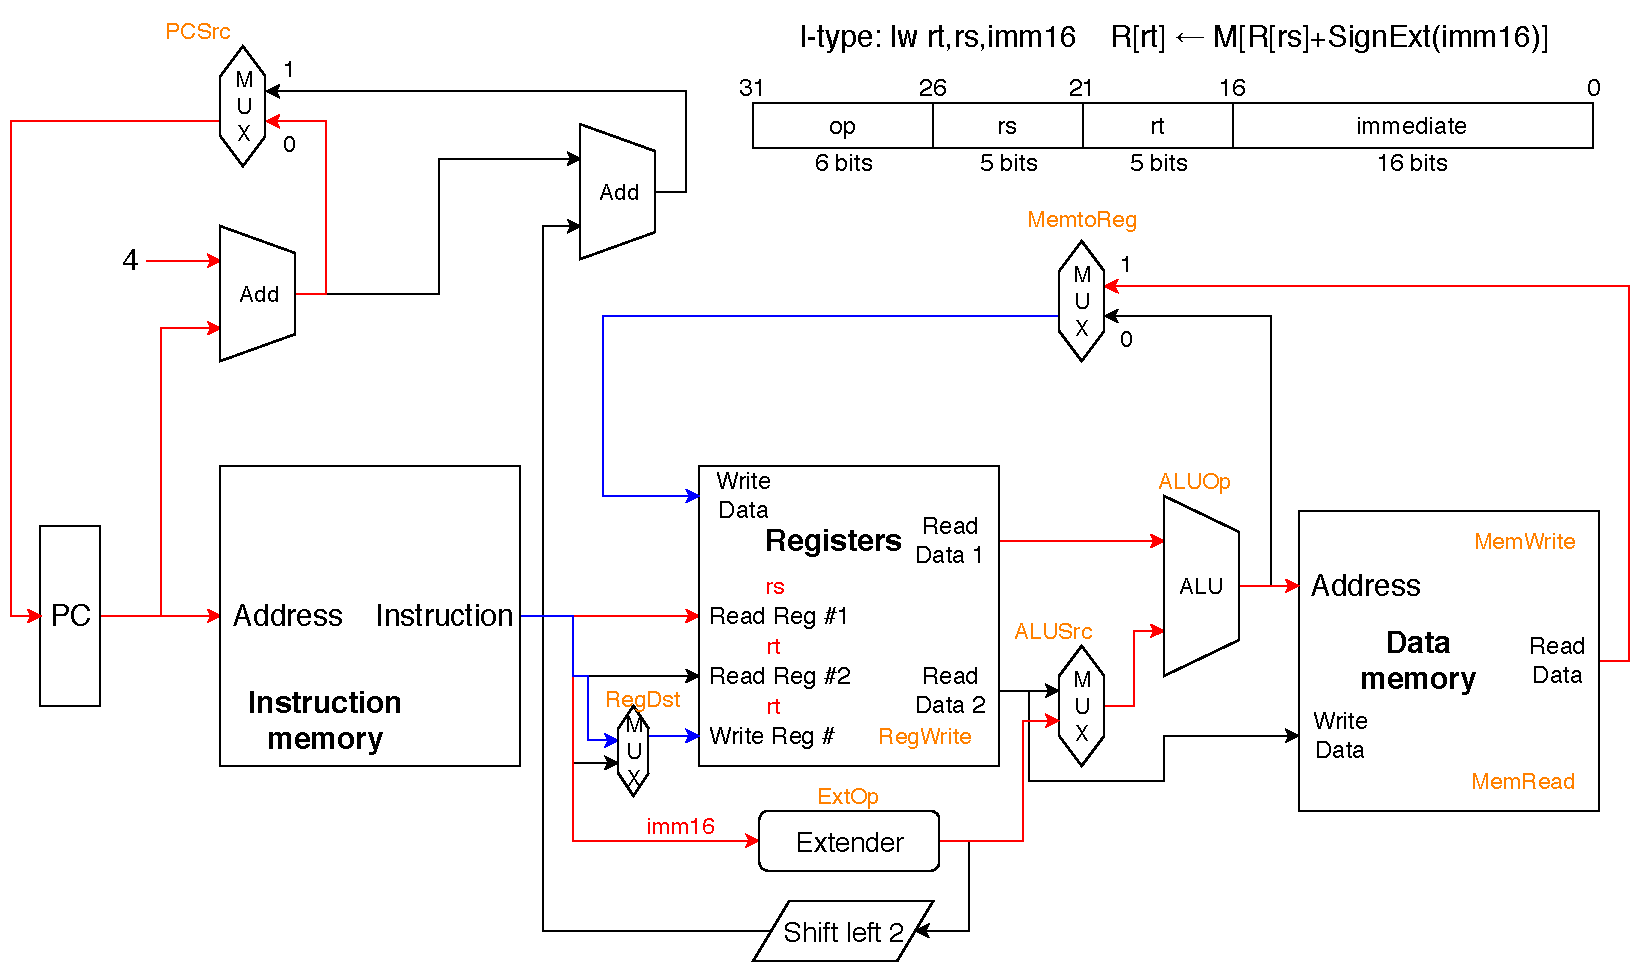
\includegraphics[width=\linewidth]{fig/Datapath_lw.pdf}
\caption{lw通路}
\end{figure}
	\item 分支 \verb'beq rs,rt,imm16':PC只需30位,因每次加4
\begin{figure}[htbp]
\centering
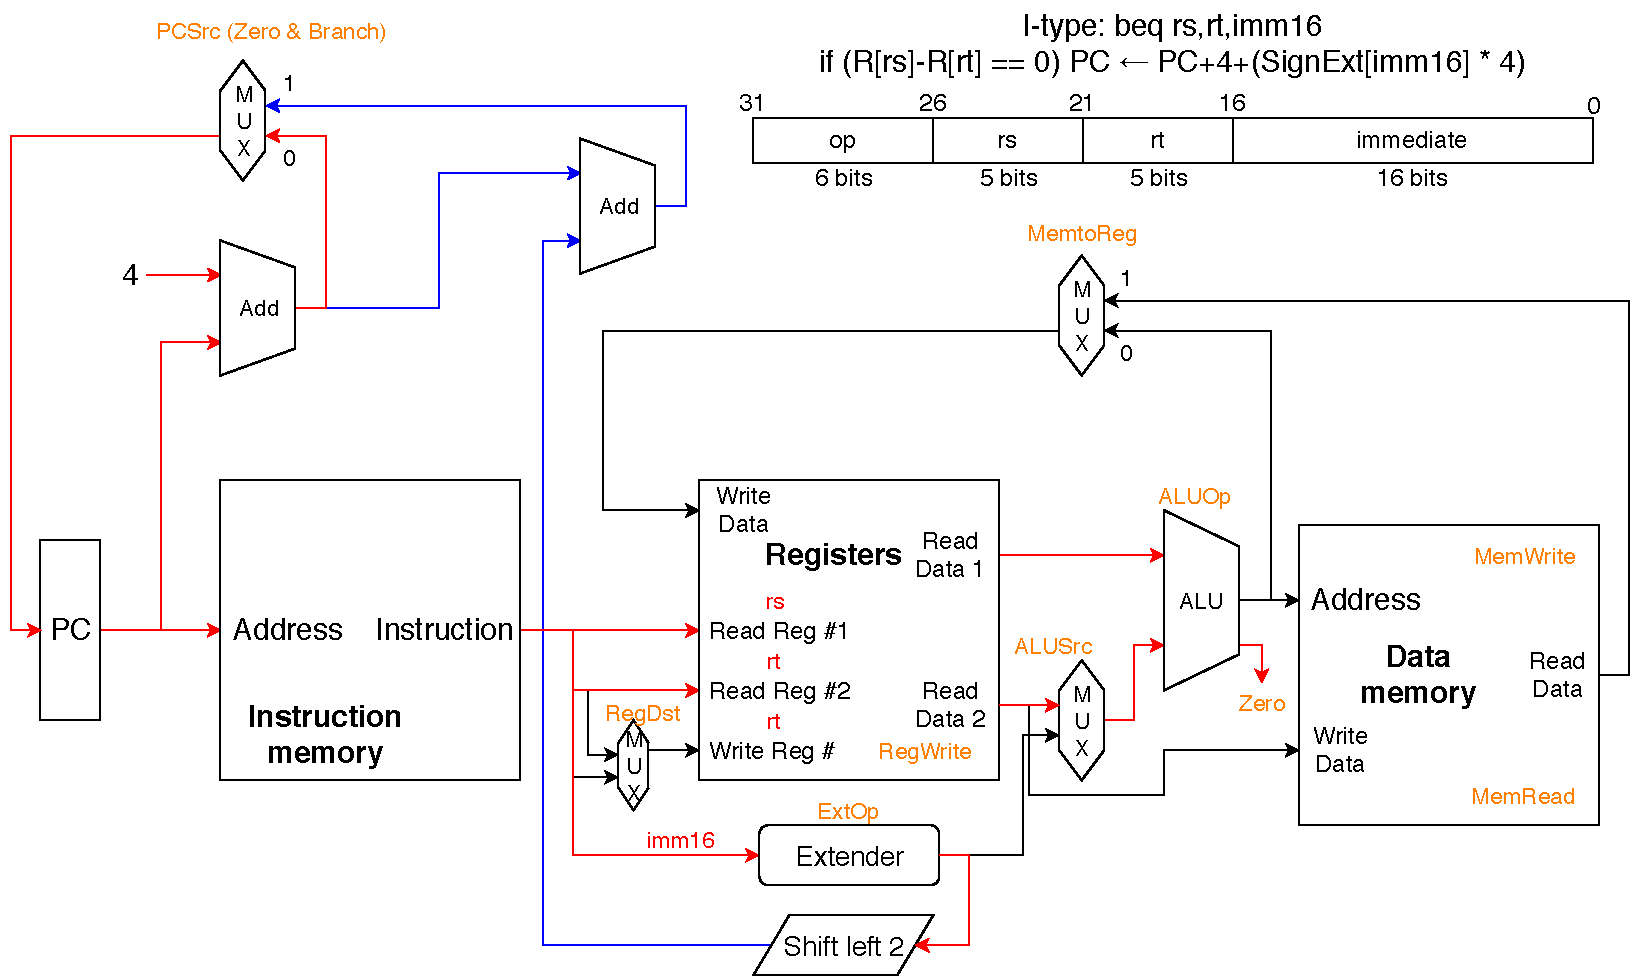
\includegraphics[width=\linewidth]{fig/Datapath_beq.pdf}
\caption{beq通路}
\end{figure}
	\item 跳转 \verb'j target':PC+4的高四位串接26位立即数然后左移2位
\begin{figure}[htbp]
\centering
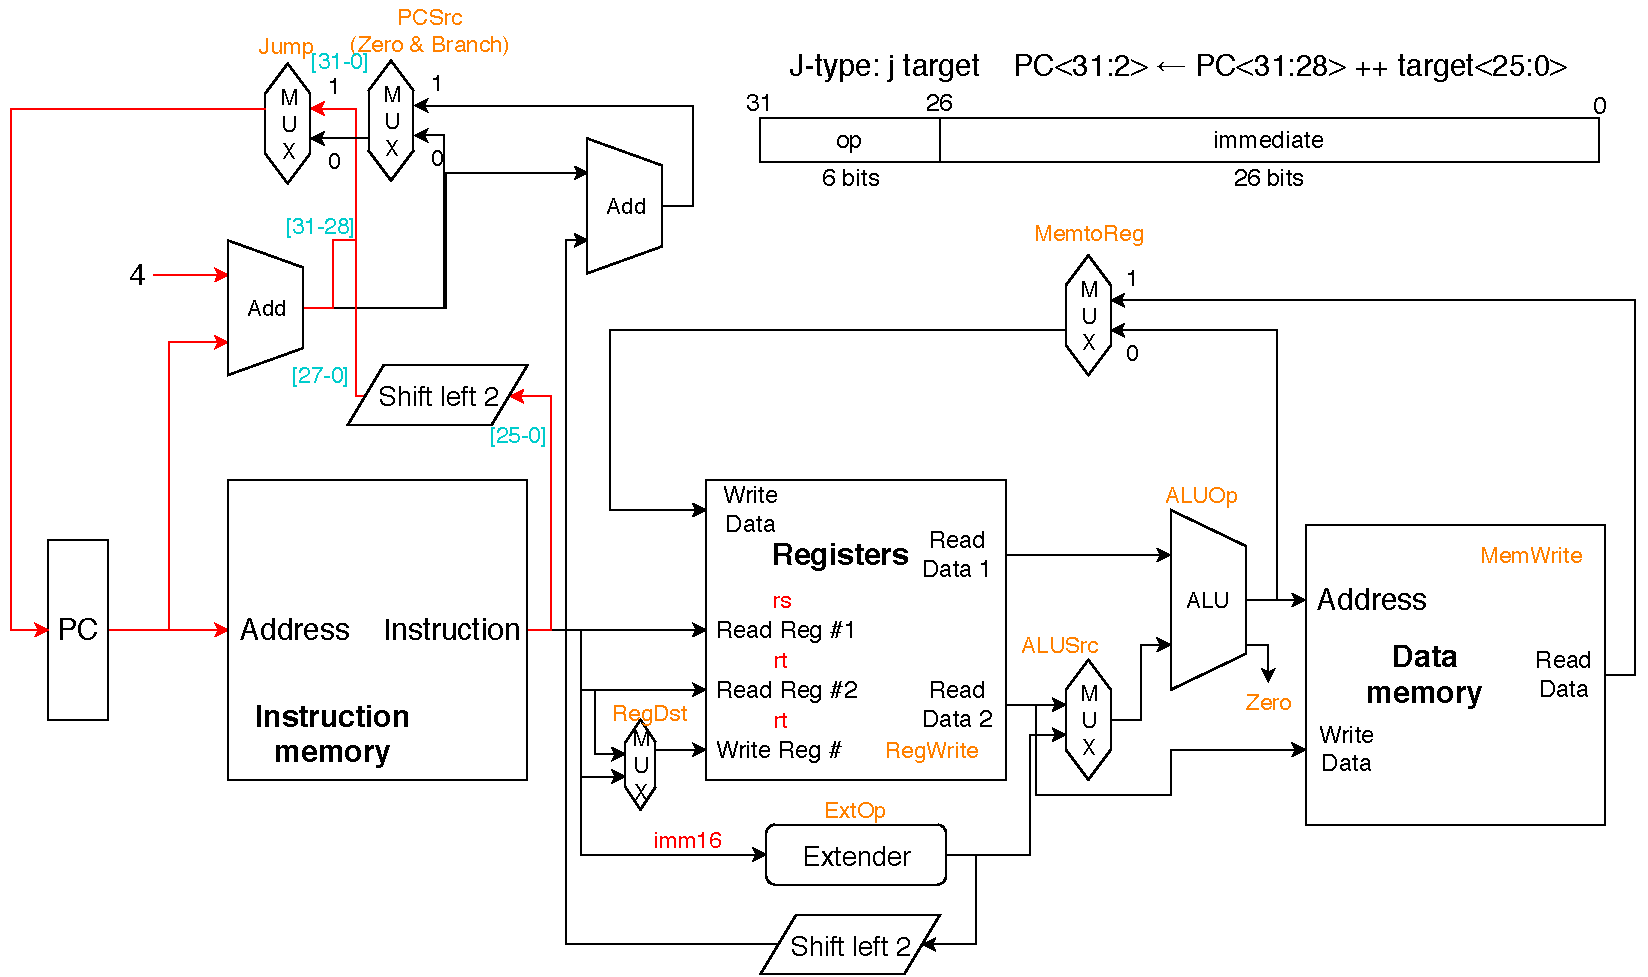
\includegraphics[width=\linewidth]{fig/Datapath_jump.pdf}
\caption{jump通路}
\end{figure}
\end{enumerate}

\subsection{多周期}
五个阶段:取指(IF)、译码(ID)、执行(EXE)、访存(MEM)、写回(WB)
\begin{itemize}
	\item 每个周期都在下个时钟到来时结束(此时存储元件被更新)
	\item 取指结束时PC+4开始写入PC,下个周期时,PC已被更新,置IRWr=0
	\item ALU空闲可用来投机计算转移地址
\end{itemize}
\begin{figure}[htbp]
\centering
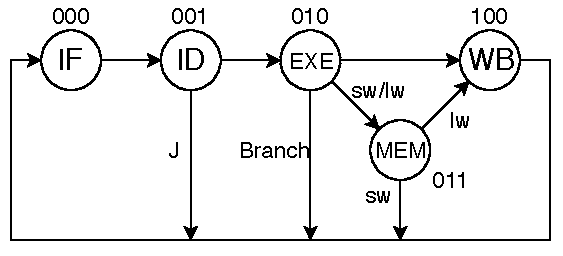
\includegraphics[width=0.5\linewidth]{fig/Datapath-Multi-cycle.pdf}
\caption{多周期CPU状态转移表}
\end{figure}
\par 注意beq3周期、lw5周期、sw4周期,而课本上jump为3周期(因将DR放在扩展器后)
\par 然而实际机器的寄存器组和存储器不一定用时钟边缘触发:
\begin{itemize}
	\item 寄存器有时钟输入,存储器可能无时钟输入
	\item 写操作不是由时钟边缘触发,而是一个组合电路:Din稳定,写使能为1,经过Write Access时间,才进行写入;会存在竞争问题
\end{itemize}

\subsection{流水线}
\subsubsection{概述}
提升工作主频:
\begin{center}
减少每个流水级执行时间$\to$减少每个流水级的任务量$\to$任务再分解$\to$增加流水线级数
\end{center}
\par 副作用:
\begin{itemize}
	\item 寄存器开销(overhead):收益下降
	\item 非均匀延迟(Nonuniform delays):吞吐率受限于最慢栈的时间,但很难将ALU和存储器划分成更小的栈
\end{itemize}
\par 流水线不能缩短时钟周期,但能减少CPI(吞吐率提升)
\par 时钟周期等于最长阶段花费时间$t$,N条指令执行时间$(5+N-1)\times t$
\par 利于流水线执行的指令集(RISC)
\begin{itemize}
	\item 指令长度一致:简化取指和指令译码
	\item 指令格式少,且源寄存器位置相同:利于在指令未知时预取操作数
	\item 只有load/store指令才能访问存储器,利于减少操作步骤,规整流水线
	\item 数据和指令在内存中\textbf{对齐}存放,利于减少访存次数和流水线规整
\end{itemize}

\subsubsection{冒险(Harzard)}
\begin{itemize}
	\item 结构冒险/资源冲突:一个功能部件同时被多条指令使用产生,如Load和R-type同时要写回
	\begin{itemize}
		\item 通过加空操作(NOP)延迟写操作(每条指令都有五个阶段)
		\item 设置多个部件(比如多个端口、寄存器读写口分开,L1级数据和指令Cache分开),避免冲突
	\end{itemize}
	\item 控制冒险/分支冒险/转移冒险:在jump/beq之前已有几条指令被取出
	\begin{itemize}
		\item 阻塞、NOP
		\item 分支预测 % 预测执行通常会发生错误,且带来很高的恢复执行代价,错的
		\begin{itemize}
			\item 静态:总是预测条件不满足,或加启发式规则
			\item 动态:根据历史情况(Branch History Table, BHT)进行调整(微型强化学习)
		\end{itemize}
		\item 指令静态调度:编译优化指令顺序,实现分支延迟
	\end{itemize}
	\item 数据冒险/数据相关:写后读
	\begin{itemize}
		\item 转发(forwarding/bypassing):将数据从流水段寄存器(EXE)/内存(MEM)中直接取到ALU的输入端(半转发/全转发),如果在Data Memory读出则无法转发(Load-use数据冒险)
		\item 阻塞(stall):插入Bubble或插入NOP
		\item 静态指令调度:编译优化指令顺序,拉大具有数据冒险指令的距离,减少流水线可能产生的停顿(可以解决load-use);也即先把后面无关的操作调到前面来执行;或者说利用闲置资源先干后面的事情(乱序执行)% 只有在半并行(流水线)才会出现?
		\begin{figure}[htbp]
		\centering
		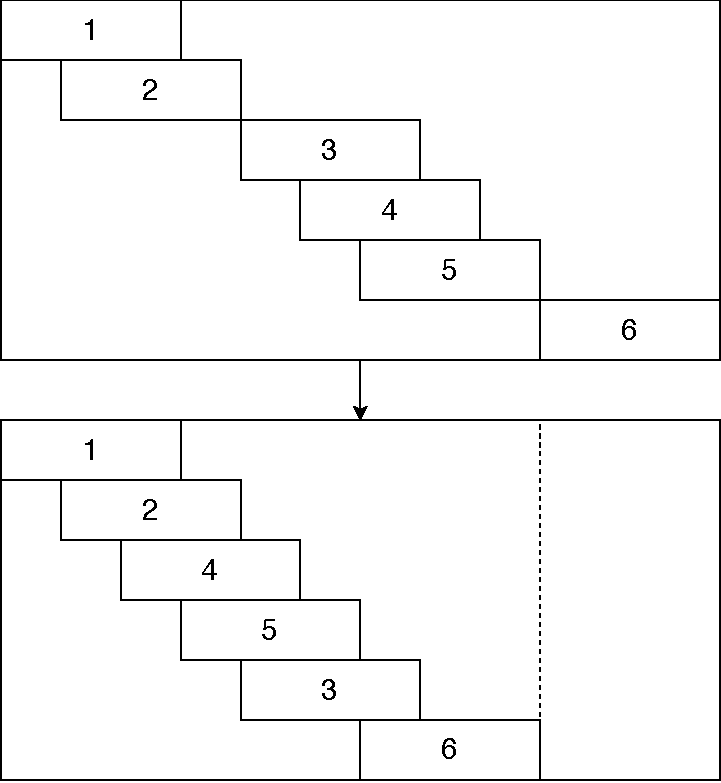
\includegraphics[width=0.3\linewidth]{fig/schedule.pdf}
		\caption{编译器调度}
		\end{figure}
	\end{itemize}
\end{itemize}

\subsubsection{指令级并行}
指令之间的相关性
\begin{itemize}
	\item 结构相关:同时存取相同寄存器或存储器
	\item 数据相关:RAW、WAR、WAW(注意中英文顺序区别)
	\item 控制相关
\end{itemize}
\par 指令级并行(ILP)技术
\begin{itemize}
	\item 静态多发射:在执行前,由编译器帮助封装多条指令并处理冒险
	\begin{itemize}
		\item 发射包:可以在给定时钟周期内发射多条指令
		\item 发射槽:在给定时钟周期内能够发射指令的位置
		\item 超长指令字(VLIW):一类可以同时启动多个操作的指令集,一条指令来实现多个操作的并行执行
	\end{itemize}
	\item 动态多发射:在运行时,由处理器发射多条指令并处理冒险
	\begin{itemize}
		\item 超标量(superscalar):一种高级流水线技术,可以使每个周期处理器能执行的指令数超过一条\\
	试图在一个周期取出多条指令并行执行,通过在处理器中内置多条流水线来同时执行多个处理。本质是以空间换取时间,在不同流水线中不相关地执行多条指令。允许指令以不同于原程序顺序的次序执行
		\item 动态流水线调度:对指令进行重新排序以避免阻塞的硬件支持
	\end{itemize}
\end{itemize}
\par 线程级并行(TLP)技术
\begin{itemize}
	\item 对于MIMD(多指令流多数据流),每个处理器执行自己的指令流
	\item 为了加大程序执行的并行力度,将程序划分为多个单一控制的执行流,每个执行流称之为一个线程。同一个进程中的不同线程共享数据空间,拥有自己的执行堆栈和程序计数器
	\item 提高系统整体的吞吐量
\end{itemize}
\par 主要技术
\begin{itemize}
	\item 超线程(Hyper-Threading)技术
	\begin{itemize}
		\item Intel Xeon(2002)
		\item 允许物理上单个处理器采用共享执行资源的方法同时执行两个或更多的分离代码流(线程), 又称\textbf{软件多线程}
		\item 把单物理处理器模拟成2个或多个逻辑处理器,每个逻辑处理器都有独立的IA-32架构,即拥有自己的通用寄存器、段寄存器、控制寄存器、调试寄存器等
		\item 减少CPU的闲置时间,提高系统的资源利用率
		\item 逻辑处理器共享的资源包括执行引擎和系统总线接口
		\item 举例:两个线程整型\&浮点、运算\&I/O
	\end{itemize}
	\item 多核(Multi-Core)技术---空间并行
	\begin{itemize}
		\item Intel Core (2006)
		\item 通过在一个物理封装中集成多个分离的完整执行核来提供\textbf{硬件多线程}能力
		\item 每个完整的执行核拥有独立的指令集、执行单元,即不仅有自己的AS,还拥有自己的执行引擎,总线接口与L2 Cache等
		\item 本质是硬件的冗余,让不同处理器并发执行不同任务
		\item 效率与性能提升要比HT技术高得多
	\end{itemize}
\end{itemize}

\subsection{异常处理}
\begin{itemize}
	\item 内部异常(Exception):CPU发生的意外事件或特殊事件
	\begin{itemize}
		\item 硬故障中断:电源掉电、硬件线路故障等;机器将\textbf{终止},调出中断程序重启操作系统
		\item 程序性中断:执行某条指令时发生的异常
		\begin{itemize}
			\item 故障:执行指令引起的异常,如溢出、缺页、访问超时
			\item 自陷:预先安排的事件,如单步跟踪、系统调用等(自愿中断),处理完回到下条指令!
		\end{itemize}
	\end{itemize}
	\item 外部中断:CPU外发生的特殊事件,外界发送中断请求信号,如打印机缺纸、外设准备好、DMA传输结束等
\end{itemize}
\par 检测到异常时,处理器需进行以下操作
\begin{itemize}
	\item 关中断:使处理器处于禁止中断状态
	\item 保护断点和程序状态:堆栈或特定寄存器
	\item 识别异常事件
	\begin{itemize}
		\item 软件识别:非向量中断(MIPS)\\
		EPC存放断点(异常处理后返回到的指令地址),总是存优先级最高的一个\\
		设置异常状态寄存器(Cause),操作系统用一个异常处理程序,按优先级顺序查询异常状态寄存器,识别出异常事件,转入相应的中断服务程序执行
		\item 硬件识别:向量中断(80x86)\\
		用专门的硬件查询电路按优先级顺序识别异常,得到“中断类型号”,到中断向量表中读取对应的中断服务程序的入口地址\\
		中断向量地址=中断类型号$\times$4
	\end{itemize}
\end{itemize}
\par 流水线中的异常处理
\begin{itemize}
	\item 在PC前的MUX加入多路输入,每路输入时一种异常程序的地址
	\item 在流水线的合适阶段(如译码、执行)添加异常检测
	\item 异常检测的输出应能控制PC前的MUX要选哪路作为输入
	\item 将出现异常的指令之后的指令全部置为NOP
\end{itemize}

\subsection{控制器}
现在常用折中方案:简单指令用硬连线,复杂指令用微控制
\subsubsection{硬连线控制器}
组合逻辑/有限状态机
\begin{itemize}
	\item 程序计数器PC
	\item 指令寄存器IR
	\item 节拍发生器Timing:有限状态机,确定指令执行顺序
	\item 控制信号产生电路CU
\end{itemize}

\subsubsection{微程序控制器}
\begin{center}
\begin{tikzcd}
\text{微程序(固件firmware)}\arrow{d}& \\
\text{微指令(一个状态, microinstruction)}\arrow{d} & \\
\text{微命令(控制信号, microcode)}\arrow{r} & \text{微操作(执行部件)}
\end{tikzcd}
\end{center}
微程序设计
\begin{itemize}
	\item 将传统的程序设计方法运用到控制器的逻辑设计中
	\item 用规整的存储逻辑代替不规则的硬接线逻辑来实现计算机控制器功能的技术
\end{itemize}
Wilkes模型(1951):输入指令寄存器IR中的操作码和机器状态标志;输出微操作控制信号\\
控制器处理一条指令的工作过程,就是启动这条指令在控制存储器中所对应的微程序,一条一条地顺序执行微指令的过程\\
微程序控制器工作过程
\begin{enumerate}
	\item IR中操作码经微程序顺序控制逻辑$\mu$C变换为该条指令微程序入口的微地址码
	\item 访问地址部件FCMAR选择微地址码,作为当前控制存储器的访问地址
	\item 根据地址从控制存储器读出一条微指令存入微指令寄存器中,其控制信号字段表示了当前运算器、存储器、控制器及FCMAR所需要执行的所有微操作
	\item 重复(2)、 (3),用微指令寄存器中地址码作为当前微地址码,直到一条指令对应的微程序执行完毕;接着执行一段微程序取下一条指令存放在IR中,然后返回(1)
\end{enumerate}
\begin{itemize}
	\item 程序计数器PC
	\item 指令寄存器IR
	\item 微指令下地址形成部件
	\item 控制存储器(只读,存放微程序)和微指令存储器
\end{itemize}
微指令格式:$\mu$OP、$\mu$Add(下条微指令地址)、常数(可选)\\
微指令编码方式:
\begin{itemize}
	\item 水平型微指令(面向控制逻辑):相容微命令尽量多安排在一条微指令中,最大限度并行
	\begin{itemize}
		\item 直接控制编码:不需译码,每个微命令用一位信息表示,易并行,但编码空间利用率低(即有多少个控制信号就多少位)
		\item 字段直接编码(显式编码):将微操作划分为若干小字段,每个字段单独编码,需译码
		\begin{itemize}
			\item 相容微操作:可同时进行,划分在不同字段
			\item 互斥微操作:不能同时进行,划分在同一字段
		\end{itemize}
		\item 字段间接编码(隐式编码):某些参与编码的微命令不能由一个控制字段直接定义,需要两个或两个以上的控制字段来定义
	\end{itemize}
	\item 垂直型微指令(面向算法):采用短格式,一条微指令只能控制一个微操作,速度慢
	\begin{itemize}
		\item 最短编码法:将所有微命令统一编码每条微指令只包含一个微命令,每次只产生一个微操作,通过译码器产生微操作控制信号;微程序长,大量译码电路,速度慢
	\end{itemize}
\end{itemize}
\begin{figure}[H]
\centering
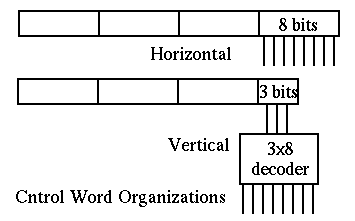
\includegraphics[width=0.4\linewidth]{fig/microinstruction.png}
\end{figure}
若机器指令共$n$条,则对应的微程序数至少$n+1$个(加一个取指微程序)
\par 微指令地址产生方法:
\begin{itemize}
	\item 顺序转移(计数器)法:下条微指令地址隐含在微程序计数器$\mu$PC中
	\item 断定(下址字段)法: 当前微指令中显式指定下条微指令地址
\end{itemize}